\chapter{自由創作}
ここまでで、基本的なテトリスの作り方を学びました。
残った部分については、自由にアレンジしてみましょう。
\section{自由創作のアイデア}
\begin{itemize}
  \item ゲームオーバーの設定
  \item スコアの計算、表示
  \item スコアに応じた落下速度の変更
  \item 4行消し(Tetris)、Tスピンなどの特殊な消し方の実装
  \item ネクストブロックの表示
  \item ホールド機能の実装
\end{itemize}
このほかにも、自分で考えたアイデアを実装してみましょう。

\section{各プログラムの構成と役割}
自由創作にあたって、各プログラムの構成と役割を確認しておきましょう。
どのプログラムがどのような役割を持っているかを把握することで、具体的にどのプログラムを変更すればよいかがわかります。

\subsection{main関数}
main関数は、ゲーム全体の流れを管理します。
以下のような変数を持っています。
\subsubsection{board変数}
Board型の変数で、盤面、カーソル、保持中のブロックを表します。
\subsubsection{screen変数}
PygameのSurface型の変数で、画面を表します。
\url{https://www.pygame.org/docs/ref/surface.html}に詳しく説明があります。
\subsubsection{clock変数}
Pygameのtime.Clock型の変数で、フレームレートを管理します。
\url{https://www.pygame.org/docs/ref/time.html#pygame.time.Clock}に詳しく説明があります。
\subsubsection{timer変数}
int型の変数で、ゲーム内の一秒を管理するために作りました。
while文の中で1ずつ増やし、60になったら0に戻します。
\begin{figure}
  [h]
  \centering
  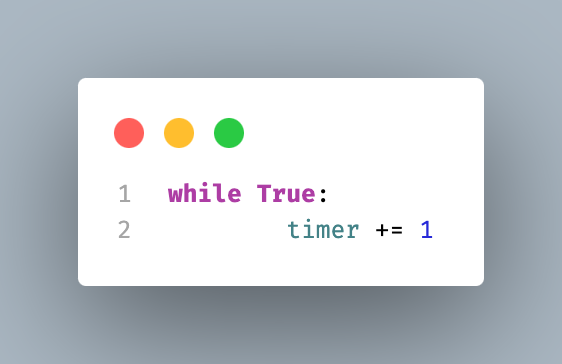
\includegraphics[width=50mm]{images/timerVar.png}
  \caption{timer変数のカウントアップ}
\end{figure}
\begin{figure}
  [h]
  \centering
  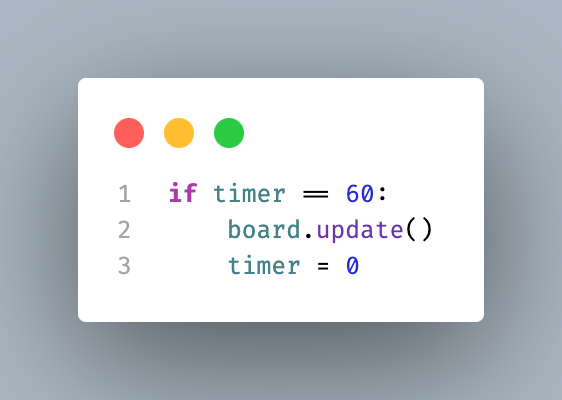
\includegraphics[width=50mm]{images/timerReset.png}
  \caption{timer変数のリセット}
\end{figure}
boardのupdate関数を呼び出しているのもここです。
ブロックの落下のタイミングを早くしたい場合は、60の部分を変数を用いたり、別の値にすると変化します。
\subsubsection{main関数の中のwhile文}
while文の中で、盤面を更新します。
また、キー入力を受け取り、board変数の関数を呼び出します。

\subsection{Boardクラス}
\subsubsection{\_\_init\_\_関数}
以下の変数を初期化します。
\begin{itemize}
  \item board変数 \newline 2次元リストで盤面を表します。中身にはブロックの色を入れています。board[y][x]で(x,y)の座標の色を取得できます。
  \item TILE\_SIZE変数 \newline マスのサイズを表します。大きくすると盤面が大きくなります。
  \item cursor変数
\end{itemize}
最後に、generate\_block関数を呼び出すことで、moving\_block変数も初期化しています。
holding\_block変数を追加すれば、ホールド機能を実装することもできます。
\subsubsection{draw関数}
保持しているboard変数を元に、盤面を描画します。
次に、cursor変数を元に、保持中のブロックとカーソルを描画します。
枠線も描画しています。

\subsubsection{window\_size関数}
ブロックのサイズを元に、ウィンドウのサイズを計算します。
pygame.display.set\_mode関数でウィンドウを作成する際に使うことを想定しています。

\subsubsection{cursor\_move\_up,down,left,right関数}
カーソルを動かす関数です。そのままcursorの関数を呼び出しています。
盤面端の判定などはCursorクラスで行なっています。

\subsubsection{block\_rotate関数}
ブロックを回転させる関数です。moving\_block変数を用いて回転の判定、実際の回転を行います。

\subsubsection{drop関数}
while文を用いて、ブロックを落下させる関数です。

\subsubsection{update関数}
main関数からtimer変数の更新関連で呼び出される関数です。
一マス落下させる処理や、一番下まで落ちた際にはブロックを固定するfix関数や、
次のblockを生成するgenerate\_block関数の呼び出し、最後に行を消去するerase\_lines関数の呼び出しを行います。

\subsubsection{fix関数}
ブロックを固定する関数です。ブロックの色をboard変数に書き込みます。
ブロックの固定先が盤面から出てしまった場合、ゲームオーバーとすることも可能です。

\subsubsection{generate\_block関数}
次のブロックを生成する関数です。カーソルの位置を上に戻した後、次のブロックをランダムに生成し、moving\_block変数に代入します。
このタイミングで、次のブロックを表示するために、next\_block変数を作成して代入すれば、次のブロックを表示することもできるかもしれません。

\subsubsection{erase\_lines関数}
行を消去する関数です。BLACKが含まれていない行を消去します。
行を消去したら、上から空の行を追加することで、盤面全体の行数が変わらないようにしています。
この際、カウンターとなる変数を用意して行を消すたびにカウンターを増やし、4だったらTetrisとすれば、Tetrisの処理を行うこともできます。
さらに、スコア変数をBoardクラス全体で持っていれば、スコアの計算も行うことができます。

\subsection{各Blockクラス}
\subsubsection{\_\_init\_\_関数}
各ブロックの色や向きを初期化します。
color変数やrotation変数を持っています。

\subsubsection{block\_info関数}
各ブロックの形を返す関数です。各ブロックの形を座標のリストで返します。
ブロックの現在位置を知るために、Cursor型の変数を引数にとります。

\subsubsection{can\_go\_up,down,left,right関数}
ブロックが移動できるかどうかを判定する関数です。
移動できる場合はTrue、できない場合はFalseを返します。
自分の位置を知るために、Cursor型の変数を引数にとり、
まわりのブロックの情報を知るためにBoard型の変数を引数にとります。

\subsubsection{can\_rotate関数}
ブロックが回転できるかどうかを判定する関数です。
回転できる場合はTrue、できない場合はFalseを返します。
自分の位置を知るために、Cursor型の変数を引数にとり、
まわりのブロックの情報を知るためにBoard型の変数を引数にとります。

\subsubsection{rotate関数}
ブロックを回転させる関数です。
実際にはrotation変数を変更しているだけで、
そのrotation変数を元にblock\_info関数で回転後の形を計算し
その値をBoardが描画し画面に反映させています。

\subsection{Cursorクラス}
\subsubsection{\_\_init\_\_関数}
カーソルの位置を初期化します。
x変数、y変数を持っています。

\subsubsection{move\_up,down,left,right関数}
カーソルを動かす関数です。
引数として取ったblockに移動可能かどうかを判定してもらい、
移動可能な場合はカーソルを移動させます。

\section{最後に}
ここまでのプログラミングで作ったクラスは以下のような関係になっています。
\begin{figure}
  [h]
  \centering
  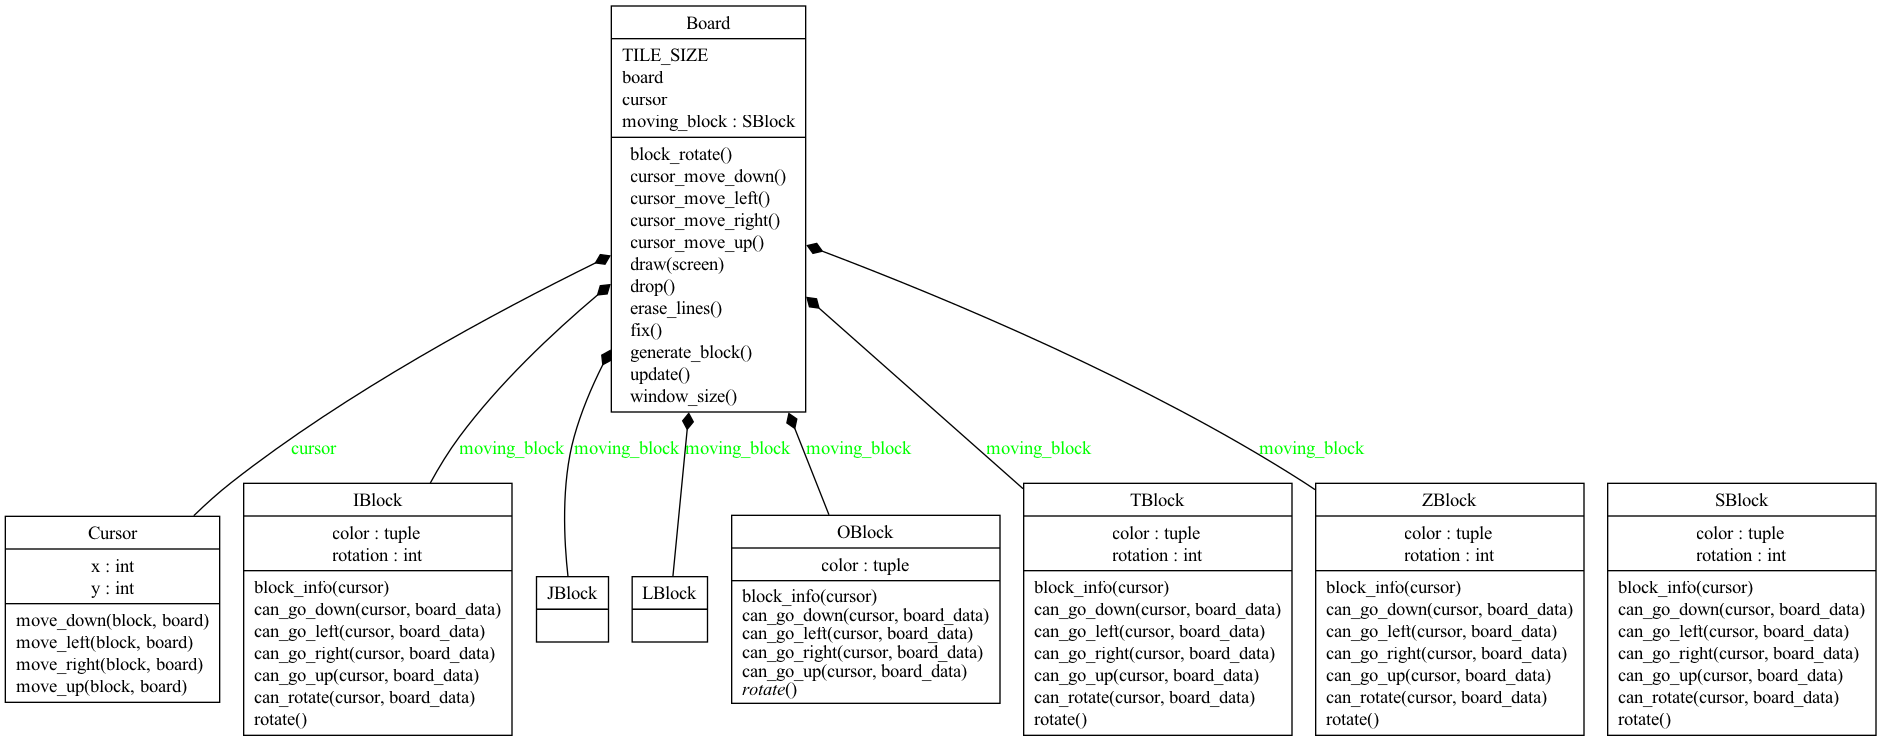
\includegraphics[width=\textwidth]{images/classes_tetris.png}
  \caption{クラス図}
\end{figure}
このような図をクラス図といいます。
\newpage
Pythonに限らず、オブジェクト指向プログラミングではこのように
クラスを作り、機能を整理し、その連携をデザインすることでプロジェクトを進めていきます。
例えば、ChromiumというGoogle Chromeなどの元となるブラウザの一部は、以下のようなクラス図を持っています。
\footnote{\url{https://www.chromium.org/developers/class-diagram-webkit-webcore-to-chrome-browser/}より引用。}
\begin{figure}
  [h]
  \centering
  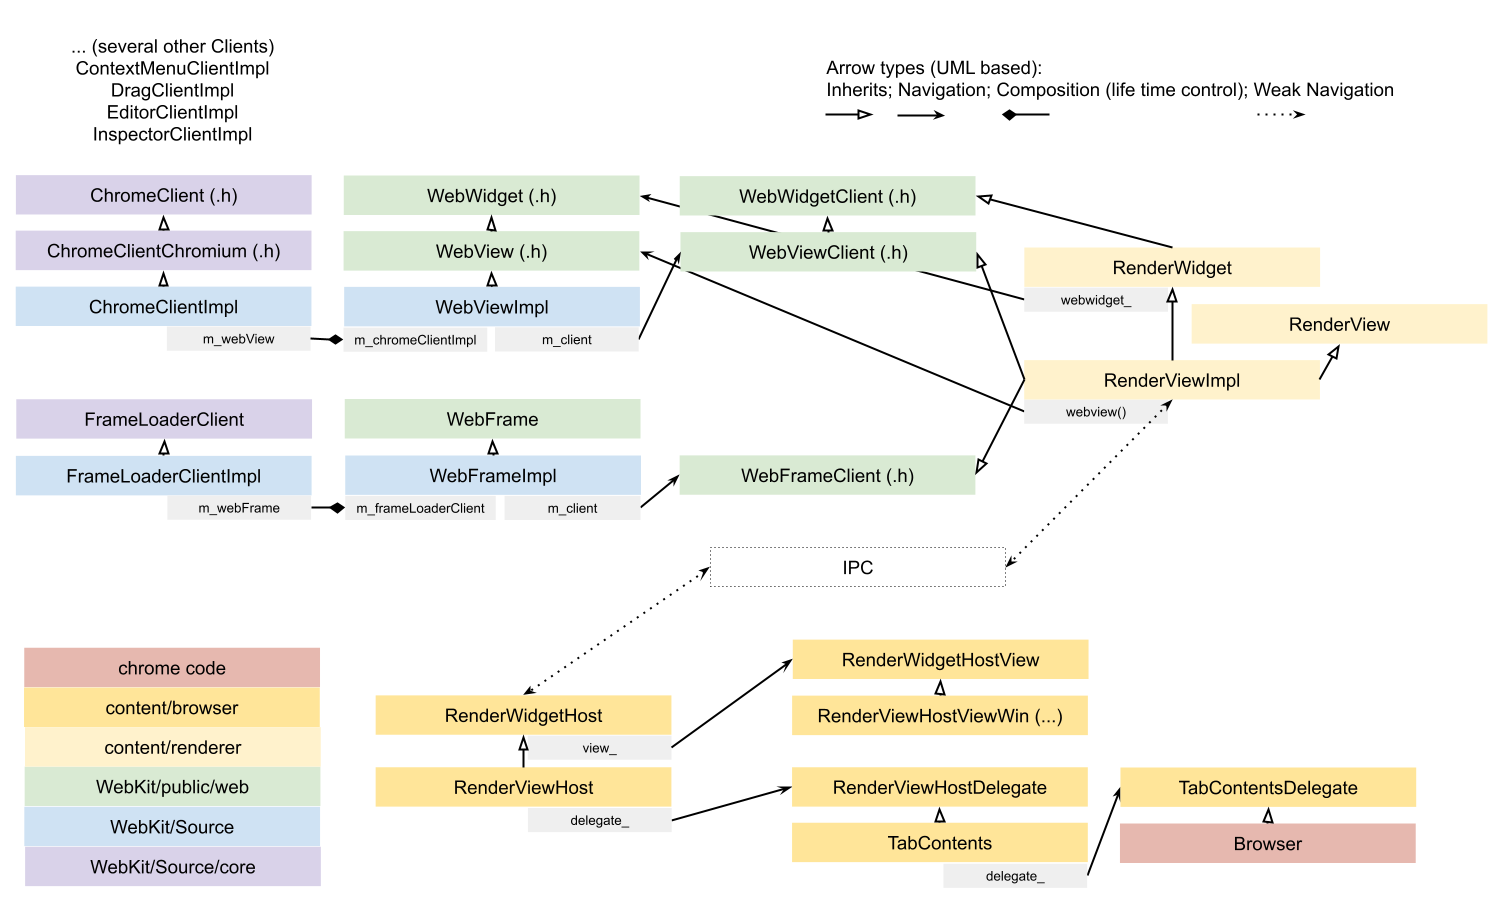
\includegraphics[width=\textwidth]{images/Chromium.png}
  \caption{Chromiumのクラス図(一部)}
\end{figure}
今回作ったものよりも複雑で、多くのクラスが連携してWebブラウザという高機能なプログラムを作っています。
しかし、簡単な機能を持ったクラスをひとつひとつ組み合わせて作っていくという考え方は同じです。

これからプログラマーになるにあたって、クラスを設計するという機会は必ずあると思います。
ぜひ、この経験を活かして自分のプログラムをより良いものにしていってください。